\documentclass[a4paper,10pt]{article}
\usepackage[utf8]{inputenc}
\usepackage{xspace}
\usepackage{graphicx,graphics} 
\usepackage{color}
\usepackage{amsmath}
\usepackage{amsfonts}
\usepackage{amssymb}
\usepackage{amsthm}
\usepackage{algorithm}
\usepackage{algorithmic}
\usepackage{longtable}
\usepackage{complexity}
\usepackage{tkz-graph}
\usepackage{float}
\usepackage{setspace}
\renewcommand{\algorithmicrequire}{\textbf{Input:}}
\renewcommand{\algorithmicensure}{\textbf{Output:}}
  
\graphicspath{{figures/}}
\newcommand\rmatching{${\cal R}$-matching\xspace}
\newcommand\mdelay{$\cal M$-delay\xspace}
\newcommand\matchedgraph{{\bf matched graph}}
\newtheorem{proposition}{Proposition}
\newtheorem{theorem}{Theorem}
\newcommand{\reporttitle}{Contention management for Deterministic Networking}     % Titre
\newcommand{\reportauthor}{Maël \textsc{Guiraud }} % Auteur
\newcommand{\reportsubject}{Master Thesis} 
\newcommand{\HRule}{\rule{\linewidth}{0.5mm}}
\setlength{\parskip}{1ex} % Espace entre les paragraphes


\newcommand{\todo}[1]{{\color{red} TODO: {#1}}}


%opening
\title{Contention Management for 5G}
\author{DB,CC,MG,OM,YS}


\begin{document}

\maketitle

\begin{abstract}
This article treats about Contention Management for 5G.
\end{abstract}

\section{Introduction}
  \itemize
    \item Context and problematic
    \item Related works
    \item Article contribution

\section{Model}

  \subsection{Definitions}
  
	We consider a symmetric directed graph $G=(V,A)$ modelling a network. Each arc  $(u,v)$ in $A$ is labeled by an integer $Dl(u,v) \geq 1$ that we call the delay and
	which represents the number of time slots taken by a signal to go from $u$ to $v$ using this arc. Note that for any arc $(u,v)$, $Dl(u,v)=Dl(v,u)$.
	
      A {\bf route} $r$ in $G$ is a sequence of consecutive arcs $a_0, \ldots , a_{k-1}$, with $a_i=(u_i,u_{i+1}) \in A$. 
      
      The {\bf latency} of a vertex $u_i$ in $r$, with $i \geq 1$, is defined by $$\lambda(u_i,r)= \sum\limits_{0 \leq j <i} Dl(a_j)$$ We also define $\lambda(u_0,r)=0$.
      The latency of the route $r$ is defined by $\lambda (r)= \lambda (u_k,r)$.
      
      A {\bf routing function} $\cal R$ in $G$ associates to each pair of vertices $(u,v)$ a route from $u$ to $v$. Let $\cal C$ be an {\bf assignment} in $G$, i.e., a set of couples of different vertices of $G$. We denote by $\cal R_{\cal C}$ the set of routes ${\cal R}(u,v)$ for any $(u,v)$ in $\cal C$. \todo{Si on s'en sert, ajouter ici que le routage est cohérent.}

   \subsection{Slotted time Model}
      Consider now a positive integer $P$ called the {\bf period}. In our problem the messages we send in the network will be periodic of period $P$ and thus we consider slices of time of $P$ discrete slots. Assume we send a message at the source of the route $r$,
      at the time slot $m$ in the first period, then a message will be sent at time $m$ at each new period. We define the first time slot at which a message reaches a vertex $v$ in this route by $t(v,r) = m + \lambda(v,r) \mod P$. 

      A message usually cannot be transported in a single time slot. We denote by $\tau$ the number 
      of consecutive slots necessary to transmit a message. Let us call $[t(v,r)]$ the set of time slots used by $r$ at a vertex $v$ in a period $P$, that is $[t(v,r)] = \{t(v,r) + i \mod P \mid 0 \leq i \leq \tau \}$.
      
      
      A {\bf $P$-periodic affectation} of $\cal R_{\cal C}$ consists in a set  ${\cal M}=(m_0, \ldots ,m_{c-1})$ of $c$ integers that we call {\bf offsets}, with $c$ the cardinal of the assignment $\cal C$. The number $m_i$ represents the index of the first slot used in a period  by the route $r_i \in {\cal R}_{\cal C}$ at its source.
      A $P$-periodic affectation must have no {\bf collision} between two routes in ${\cal R}_{\cal C}$, that is $\forall (r_i, r_j) \in {\cal R}_{\cal C}^2, i \neq j$, % with $\tau$ the size (in number of consecutive slots) of each message that must be periodically sent on each route of ${\cal R}_{\cal C}$, 
      we have $$[t(u,r_i)] \cap [t(u,r_j)] = \emptyset .$$
      
   \subsection{Problems}

      The main theoretical problem we have to deal with in this context is the following.\\

      \noindent {\bf Problem  Periodic Routes Assignment (PRA)} 

      \noindent {\bf Input:} a graph $G=(V,A)$, a set $\cal C$ of pair of vertices, a routing function $\cal R$ and an integer $P$.

      \noindent {\bf Question:} does there exist a $P$-periodic affectation of $\cal C$ in $(G,{\cal R})$?

      We will prove in Sec.~\ref{sec:complexity} that the Problem PRA is $\NP$-complete, even in restricted settings.
      In fact, even approximating the smallest value of $P$ for which there is a $P$-periodic assignment is hard.\\
% 
%       \begin{figure}[H]
%       \label{could-ran}
%       \begin{center}
%       % \begin{tabular}{cc}
%       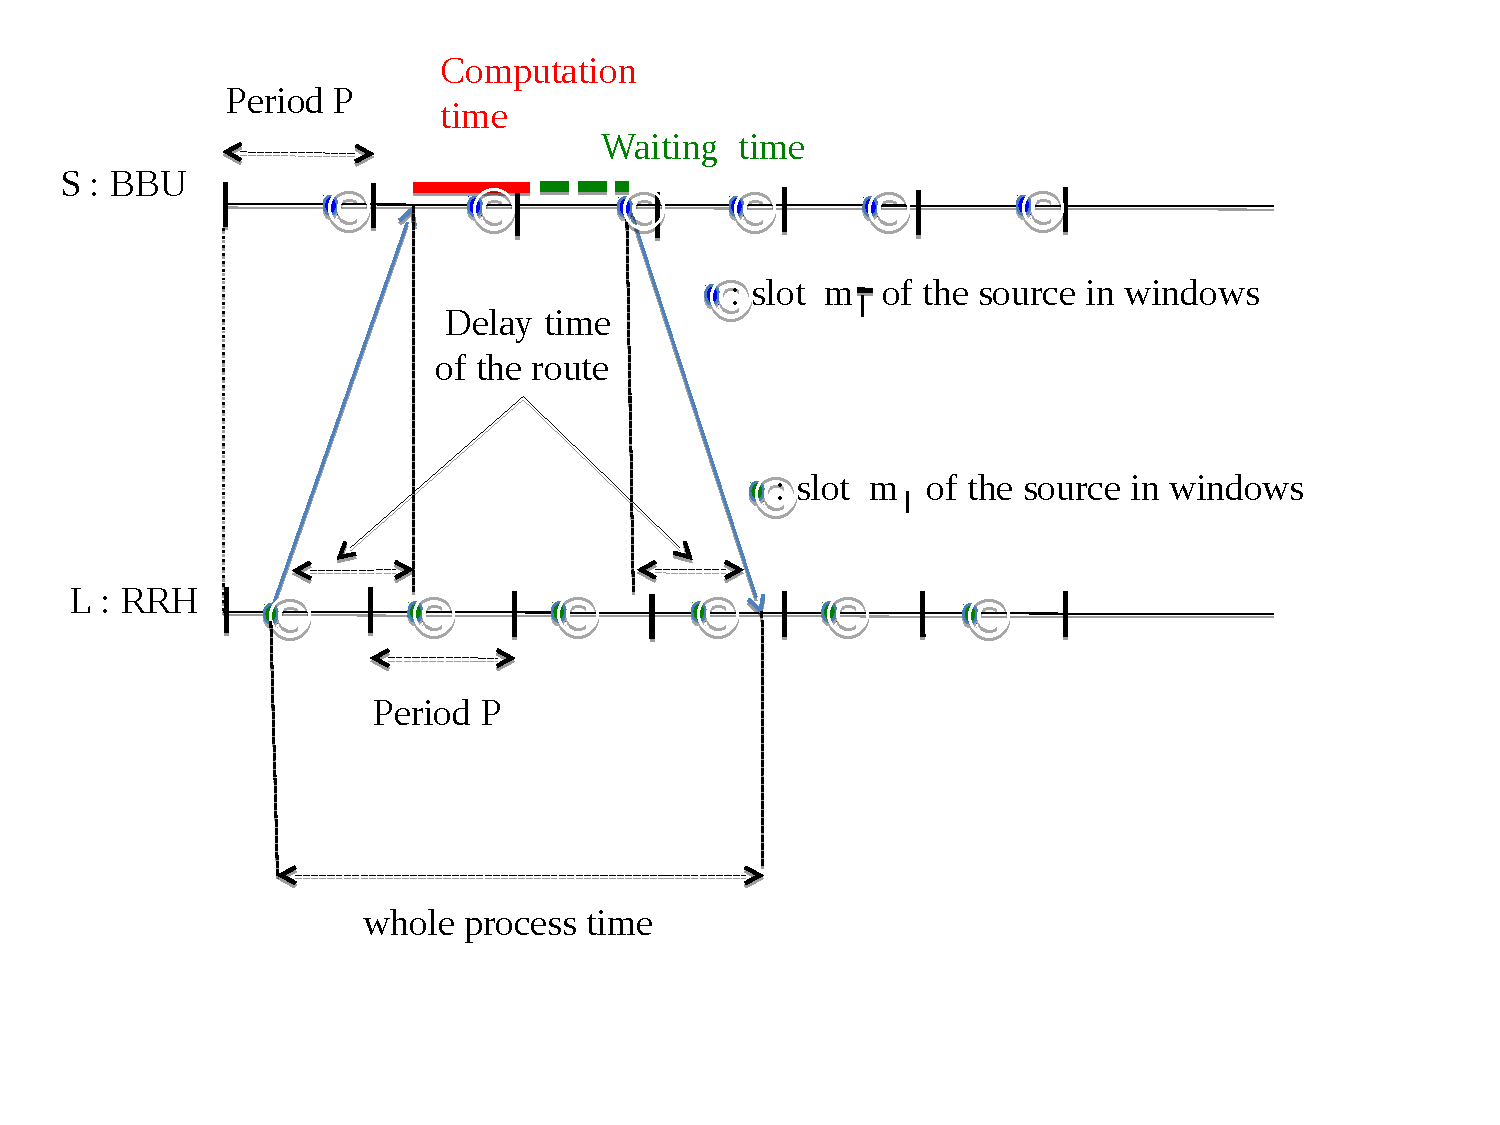
\includegraphics[scale=0.5]{Total-latence.pdf}
%       \caption{Complete process for a leaf in $L$.}
%       \end{center}
%       \end{figure}
%       %\end{tabular}\newline

      
      In the context of cloud-RAN applications, we consider here the digraph $G=(V,A)$ modeling the target network 
      and two disjoint subsets of vertices $S$ and $L$, where $S$ is the set of BBU and $L$ is the set of RRH. 
      We denote by $n$ the size of $S$ and $L$. We are given a period $P$, a routing function ${\cal R}$ and a bijection $\rho:L\rightarrow S$ which assigns a BBU to each RRH. Let ${\cal C}_{\rho} = \{(l,\rho(l))\}_{l \in L} \cup \{(s,\rho^{-1}(s))\}_{s \in S}$. Let consider a $P$-periodic affectation of ${\cal C}_{\rho}$ which associates $m_l$ to 
      $(l,\rho(l))$ and $m_{\rho(l)}$ to $(\rho(l),l)$.  
      
      This affectation represents the following process: first a message is sent in $l$, through the route $r_l$, at time $m_l$.
      This message is received by $\rho(l)$ at time $t(\rho(l),r_l)$. It is then sent back to $l$ at time $\bar{m_l}$,
      which is in the same period if $m_{\rho(l)} > t(\rho(l),r_l)$ otherwise it is in the next. The time between the arrival of
      the message and the time it is sent back is called the \textbf{waiting time} and is defined by $w_l = m_{\rho(l)} - t(\rho(l),r_l)$ if $m_{\rho(l)} > t(\rho(l),r_l)$ and $w_l = m_{\rho(l)} + P - t(\rho(l),r_l)$ otherwise.
      When a BBU receives a message, it must compute the answer before sending it back to the BBU. This time is taken into account
      in the last arc leading to the BBU and thus we need not to consider it explicitely in our model.
    
      Thus, the whole proccess time for a vertex $l$ is equal to
      $$
      PT(l)=\lambda(r_l)+ w_l+\lambda(r_{\rho(l)}).
      $$
      
    The {\bf maximum process time} of the $P$-periodic affectation ${\cal M} $ is defined by $MT({\cal M})=\max\limits_{l \in L} PT(l)$. The problem we want to solve is the following. 

      \noindent {\bf Problem Periodic Assignment for Low Latency(PALL)} 

      \noindent {\bf Input:}  a digraph $G$, a matching $\rho$ from $L$ to $S$ two disjoint set of vertices of $G$, a routing function $\cal R$, a period $P$, an integer $T_{max}$.

      \noindent {\bf Question:} does there exist a $P$-periodic affectation ${\cal M}$ of ${\cal C}_{\rho}$ in $(G,{\cal R})$ such that $MT({\cal M}) \leq T_{max}$?

      %The related optimisation problem we will focus on  consists in minimizing  $MT({\cal M})$. Note that in the context of cloud-RAN networks, we consider $P=1ms$, $\theta=2.6ms$ and $T_{max}$ must be less or equal to $3ms$.
      %cette remarque doit être dans la partie expérimentale


	

  
\section{Solving PRA}
  \label{sec:complexity}
  \subsection{NP-Hardness}
	
   \todo{Definition of the load. La preuve se réfère à la précédente qui n'a pas été retenue, il faut du coup tout expliquer.}
   
   
    \begin{theorem}
    Problem PRA cannot be approximated within a factor $n^{1-o(1)}$ unless $\P = \NP$ even when the load is two
    and $n$ is the number of pairs in the assignment.
    \end{theorem}

    \begin{proof}
    We reduce PRA to graph coloring. Let $G$ be a graph instance of the $k$-coloring problem. 
    We define $H$ in the following way: for each vertex $v$ in $G$, there is a route $r_v$ in $H$.
    Two routes $r_v$ and $r_u$ share an edge if and only if $(u,v)$ is an edge in $G$ and this edge is only in this two routes. 
    We put a weight inbetween shared edges in a route so that there is a delay $k$ between two such edges. 
    
    As in the previous proof, a $k$-coloring of $G$ gives a $k$-periodic schedule of $H$
    and conversly. Therefore if we can approximate the value of PRA  within a factor $f$,
    we could approximate the minimal number of colors needed to color a graph within a fator $f$, 
    by doing the previous reduction for all possible $k$. The proof follows from the hardness of approximability
    of finding a minimal coloring~\cite{zuckerman2006linear}.
    \end{proof}


   
  \subsection{MIN-PRA}
    Exemple de cas simple
    
\section{Proposed Solutions, solving PALL}
  
  In this section, we consider a particular case of the model, in which for each $(u,v)$ , the route is the same in both directions. This means that ${\cal R}(u,v)$ uses the same arcs as ${\cal R}(v,u)$ in the opposite orientation.
  \subsection{Intro}
    PALL NP-Hard car PRA NP-Hard\\
    Résultats valables sur Topologie 1 avec nos paramètres
    \todo{J'ai viré star affectation, car je pense qu'il n'y a rien à dire là dessus.}
    
  \subsection{No waiting times}
    \subsubsection{Shortest-longest}
      \paragraph{Algo}
      \paragraph{Period}
    \subsubsection{Greedy Algorithm with higher bound}
      \paragraph{Algo}
	Todo
      \paragraph{Period}
	This algorithm gives us a solution without waiting times in a maximum period $3.\tau.N$, if we have N routes.\\
	Suppose that we have a period of $3.\tau.N$ slots, divided in $\tau$ macro-slots.
    \subsubsection{Exhaustive generation}
      Décrire l'algo, expliquer les coupes
    \subsubsection{Results}
      Resultats des simulations : Shortest-longest optimal pour ces parametres.
      
   \subsection{Allowing waiting times}
     \subsubsection{Intro}
	Importance des waiting times quand la période est donnée (Résultats D'éxepriences et preuve avec l'exemple)
     \subsubsection{LSG}
	\paragraph{Algorithm}
	\paragraph{Analysis}
	  Parler de LSO et expliquer pourquoi LSG mieux avec nos params
     \subsubsection{Results}
	 \paragraph{Random}
	 \paragraph{Distributions}
   
\section{Conclusion}

\end{document}
